\documentclass[11pt]{article}
\usepackage{fullpage,amsthm,amsfonts,amssymb,epsfig,amsmath,times,algorithm,algorithmic}
\usepackage[table,xcdraw]{xcolor}

\newtheoremstyle{indented-remark}
{}
{}
{\addtolength{\leftskip}{2.5em}}
{}
{\bfseries}
{:}
{.5em}
{}

\newtheoremstyle{indented-proof}
{}
{}
{\addtolength{\leftskip}{2.5em}}
{}
{\slshape}
{.}
{.5em}
{}

\theoremstyle{definition}
\newtheorem{theorem}{Theorem}
\newtheorem{lemma}{Lemma}
\newtheorem{corollary}{Corollary}
\newtheorem{observation}{Observation}
\newtheorem{definition}{Definition}

\theoremstyle{plain}
\newtheorem{claim}{Claim}

\theoremstyle{indented-remark}
\newtheorem{case}{Case}

\theoremstyle{indented-proof}
\newtheorem*{proofofcase}{Proof of Case}

\begin{document}

\begin{center}
{\bf\Large CMPS 102 --- Fall 2018 ---  Homework 1}
\end{center}

\begin{center}
\textit{"I have read and agree to the collaboration policy." - \textbf{Kevin Wang}}
\end{center}

\section*{Solution to Problem 1: Truthfulness}

Given a stable matching problem with 3 women and 3 men, let a woman be Alice and three men be Ben, Carl, and David. We must prove two claims.

\begin{claim} 
If Alice prefers Ben to Carl but lies that she prefers Carl to Ben, it is possible that she can be matched with David, whom she prefers to both Ben and Carl.
\end{claim}

\begin{proof} 
There is a preference list where Alice lies that results in a stable matching where she is partnered with David.

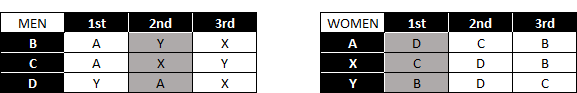
\includegraphics[scale=1]{images/fig1.png}
\end{proof}

\begin{claim} 
If Alice had been truthful in her preferences, she would not have been matched with David.
\end{claim}

\begin{proof}
The preference list where Alice is truthful does not result in a stable matching where she is partnered with David.

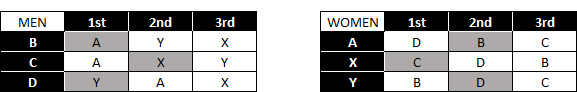
\includegraphics[scale=1]{images/fig2.png}
\end{proof}
\noindent Therefore, when running Gale-Shapley, truthfulness matters. In a man-optimal/women pessimal stable matching problem, women can benefit from lying about their preferences and get a partner they prefer more.

\end{document}